\documentclass{article} 
%All documents start with this
% This is called the preamble. It sets up the format of the document.
% It includes author information, dates, formatting etc.
% If we require any additional formatting etc, we can import ‘packages’.
% This will give us more customability.
% For exmaple: ams* packages gives us a range of symbols etc.
\usepackage{color}
\usepackage{graphicx}
\usepackage{amsmath, amsthm, amsfonts, amssymb}
% fancyhdr is a package that deals with headers and footers.
\usepackage{fancyhdr}
\setlength{\headheight}{15pt}
\pagestyle{fancyplain}
% Header and Footer content
\lhead{\today}
\chead{\LaTeX{} Primer}
\rhead{Hubert Hao}
\lfoot{left footer}
\cfoot{center footer}
\rfoot{right footer}
% Preamble ends here
\begin{document}

\title{My First Document}
\author{My Name}
\date{\today}
\date{November 2013}
\maketitle

\pagenumbering{roman}
\tableofcontents
\listoffigures
\listoftables
\newpage
\pagenumbering{arabic}


% This is where the content starts, after this line.
This is the start of a \LaTeX primer....
% Write all the content here, before this line.
\section{section}
You should divide your document into chapters (if needed), sections and subsections. The following sectioning commands are available for the article
class
\subsection{subsection}
You should divide your document into chapters (if needed), sections and subsections. The following sectioning commands are available for the article
class
\subsubsection{subsubsection}
You should divide your document into chapters (if needed), sections and subsections. The following sectioning commands are available for the article
class
\paragraph{paragraph}
You should divide your document into chapters (if needed), sections and subsections. The following sectioning commands are available for the article
class
\subparagraph{subparagraph}
You should divide your document into chapters (if needed), sections and subsections. The following sectioning commands are available for the article class



{\section{Font Size}}
\noindent
{\tiny tiny words} tiny words\\
{\scriptsize scriptsize words} scriptsize words\\
{\footnotesize footnotesize words} footnotesize words\\
{\small small words} small words\\
{\normalsize normalsize words} normalsize words\\
{\large large words} large words\\
{\Large Large words} Large words\\
{\LARGE LARGE words} LARGE words\\
{\huge huge words} huge words\\
{\Huge Huge words} Huge words\\

\noindent
\textit{words in italics} words in italics\\
\textsl{words slanted} words slanted\\
\textsc{words in smallcaps} words in smallcaps\\
\textbf{words in bold} words in bold\\
\texttt{words in teletype} words in teletype\\
\textsf{sans serif words} sans serif words\\
\textrm{roman words} roman words\\
\underline{underlined words} underlined words\\

\noindent
{\color{red}fire}

{\section{Punctuation section}}
quotes '', ', `', ``''\\
doublequoets ", `"`


{\section{Table section}}
show tables
\begin{table}[h]
  \centering
  \begin{tabular}{lcc}
    galaxy & magnitude & redshift \\
    NGC 891 & 15.5 & 0.02 \\
    M87 & 14.8 & 0.01		
  \end{tabular}
  \caption{table about planet}
  \label{tab-withoud-line}	
\end{table}


\begin{table}[h]
  \centering
  \begin{tabular}{|l|c|c|}
    galaxy & magnitude & redshift \\
    \hline
    NGC 891 & 15.5 & 0.02 \\
    \cline{2-3}
    M87 & 14.8 & 0.01		
  \end{tabular}
  \caption{table about universe}
  \label{tab-with-line}	
\end{table}




{\section{Image section}}

\begin{figure}[hp]
  \centering
  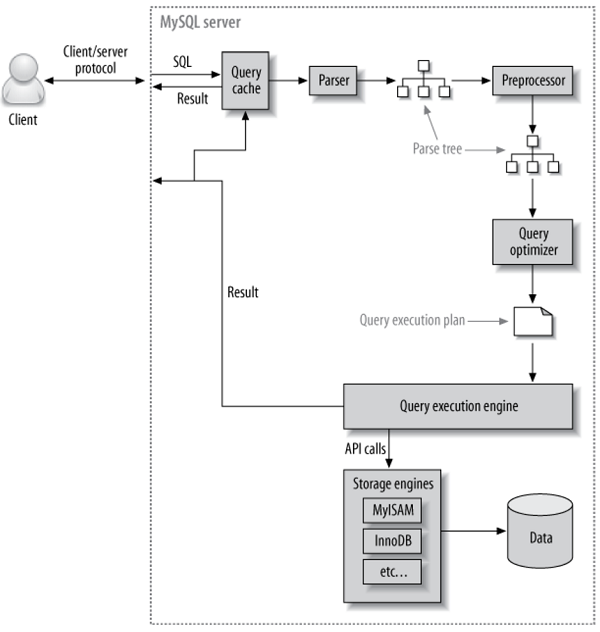
\includegraphics[width=1\textwidth]{test}
  \caption{Here is my image}
  \label{image-myimage}
  \end{figure}


{\section{Math section}}


\begin{equation}
  P_{r-j} = 
  \left\{
      \begin{array}{cl}
      0& \text{if $r-j$ is odd},\\
      r!\,(-1)^{(r-j)/2}& \text{if $r-j$ is even}.\\
        \end{array}
  \right.
  \end{equation}

\begin{equation}
  P_{r-j}=\begin{cases}
    0& \text{if $r-j$ is odd},\\
    r!\,(-1)^{(r-j)/2}& \text{if $r-j$ is even}.
    \end{cases} 
  \end{equation}

\begin{gather}
  first equation\\
  \begin{split}
  second & equation\\
  & on two lines
  \end{split}
  \\
  third equation
  \end{gather}

\begin{equation}
  g(t) = \left\{\frac{t+2}{t-3}\right\}\left(\frac{1}{t}\right)
  \end{equation}



\begin{equation}
  \begin{aligned}
    f(x) &= \frac{x^3-2x^2-11x+12}{x^2-5x+4} & {}\\
    &= \frac{(x-1)(x^2-x-12)}{(x-1)(x-4)} & {Factoring}\\
    &= \frac{(x-1)(x+3)(x-4)}{(x-1)(x-4)} & {\rm Factoring} \\
    &= x+3 &{}
  \end{aligned}
  \end{equation}    

  \begin{equation}
    \begin{aligned}
      f(x) &= \frac{x^3-2x^2-11x+12}{x^2-5x+4} \\
      &= \frac{(x-1)(x^2-x-12)}{(x-1)(x-4)} \\
      &= \frac{(x-1)(x+3)(x-4)}{(x-1)(x-4)} \\
      &= x+3
      \end{aligned}
  \end{equation}
  


\begin{enumerate}
  \item The first thing goes here.
  \item The second thing goes here.
  \end{enumerate}


\begin{itemize}
  \item The first thing goes here.
  \item The second thing goes here.
  \end{itemize}


\begin{equation}
  f(t) = 
  \left\{
    \begin{array}{cl}
      f_1(t) & x < 10\\
      x^4-x +2 & x \geq 10\\
      \frac{5}{t} & {\rm otherwise}
    \end{array}
  \right.
  \end{equation}

  \begin{equation}
    f(x) = \begin{cases}
    2x+c\sin(x) & \mbox{if } x\geq\pi \\
    cx^3-x & \mbox{if } x<\pi
    \end{cases}
    \end{equation}


$
\mathbb{Z}\\
\mathbb{N}\\
\mathbb{Q}\\
\mathbb{R}\\
\in\\
\infty\\
\alpha, \beta, \gamma\\
\delta, \pi\\
x_i\\
x^i\\
\frac{1}{x}\\
\neq\\
\geq\\
\leq\\
\pm\\
\binom{n}{k}\\
\dotsc\\
\dotsb\\
\dotsm\\
\dotsi\\
\dotso\\
$







\end{document}